% !TeX encoding = UTF-8
% !TeX root = ../main.tex

\section{研究背景及动机}

\begin{frame}{编译器的中间语言}
  \textcolor{MediumBlue}{延续传递风格(CPS)}
  \begin{itemize}
    \item CPS是\textcolor{Maroon}{函数式}编译器中常用的中间语言(IR)。
    \item 每一步计算和控制流跳转都要被\textcolor{Maroon}{显式命名}。
    \item CPS中间语言有利于进行\textcolor{Maroon}{控制流分析}。
  \end{itemize}
  \textcolor{MediumBlue}{静态单赋值(SSA)}
  \begin{itemize}
    \item SSA是\textcolor{Maroon}{LLVM、GCC}等主流编译器基础设施常用的中间语言。
    \item 每一个变量都只能被\textcolor{Maroon}{赋值一次}。
    \item SSA中间语言有利于进行\textcolor{Maroon}{数据流分析}。
  \end{itemize}
\end{frame}

\begin{frame}{编译器的中间语言}
    \begin{itemize}
      \item SSA程序可以用函数式程序表示。
      \item 目前\textcolor{Maroon}{没有}从CPS到SSA经过形式化验证的转换。
    \end{itemize}
    \begin{figure}
      \centering
      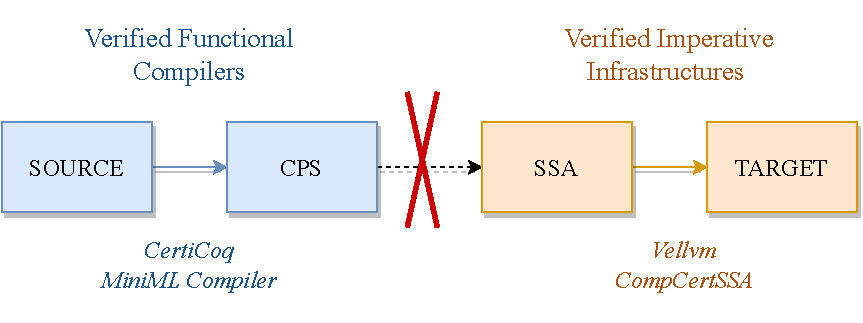
\includegraphics[width=0.7\linewidth]{figures/Motivation.drawio.pdf}
      \label{fig:moti1}
    \end{figure}
\end{frame}

\begin{frame}{研究课题概述}
  \begin{itemize}
    \item 实现并验证CPS到SSA语言的转换算法。
    \item 可以使经过形式化验证的函数式语言编译器复用基于SSA语言的优化。
  \end{itemize}
  \begin{figure}
    \centering
    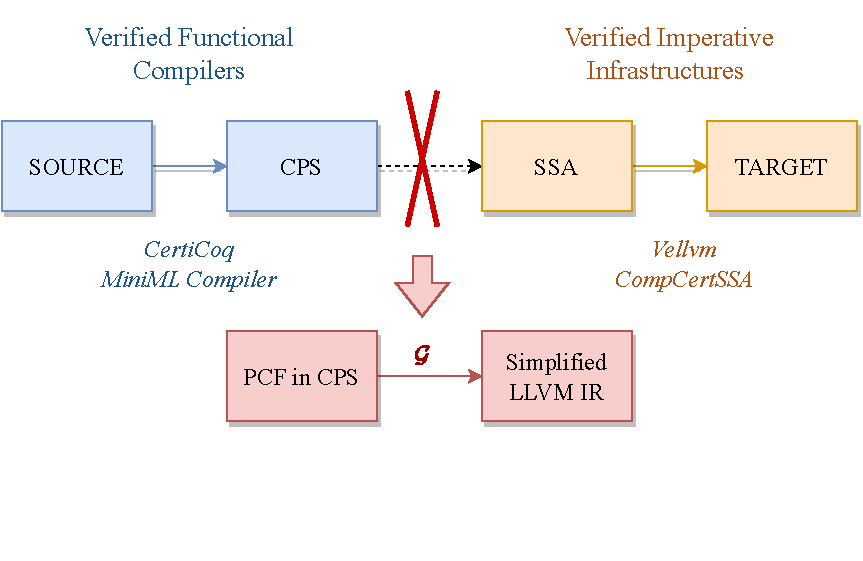
\includegraphics[width=0.7\linewidth]{figures/partial.drawio.pdf}
    \label{fig:moti2}
  \end{figure}  
\end{frame}
